\documentclass[10pt,a4paper]{article}
\usepackage[margin=1.7cm]{geometry}
\usepackage[T1]{fontenc}
\usepackage{lmodern,microtype,booktabs,graphicx,amsmath,siunitx,hyperref,caption,subcaption}
\usepackage{tikz}
\usetikzlibrary{positioning,arrows.meta,fit,backgrounds}
\captionsetup{font=small,skip=3pt}
\hypersetup{colorlinks=true, linkcolor=black, urlcolor=blue!60!black}
\setlength{\parskip}{2pt}\setlength{\parindent}{0pt}

% ------------------------------------------------------------------
% Numbers used in the text and tables
% ------------------------------------------------------------------
\newcommand{\videolink}{\url{https://youtu.be/2bmPeDtzU-s}}
\newcommand{\gitRepo}{https://github.com/AdrianMaslak/embedded_neural_network}
\newcommand{\gitHW}{\href{\gitRepo/tree/main/vivado}{\texttt{hls/}, \texttt{vivado/}}}
\newcommand{\gitSW}{\href{\gitRepo/tree/main/firmware}{\texttt{firmware/}, \texttt{pc/}}}
% software / C-simulation results (test set, 1200 images)
\newcommand{\cnnKerasAcc}{100.0}
\newcommand{\snnFloatAcc}{98.58}
\newcommand{\snnIntAcc}{97.92}
% HLS synthesis @ 100 MHz
\newcommand{\cnnLatCyc}{283\,902} \newcommand{\cnnLatUs}{2\,839}
\newcommand{\snnLatCyc}{19\,812}  \newcommand{\snnLatUs}{198}
% board measurements (pc/app.py eval, 1200 test images, 16.11.2026)
\newcommand{\cnnBoardAcc}{100.0} \newcommand{\snnBoardAcc}{97.92}
\newcommand{\cnnIpUs}{2\,840}    \newcommand{\snnIpUs}{197}
\newcommand{\cnnPreUs}{289}      \newcommand{\snnPreUs}{1\,827}
\newcommand{\uartMs}{12.0}       \newcommand{\rttMs}{30.7}

\title{\vspace{-1.2cm}Assignment 2: Accelerated AI for Vision -- CNN vs.\ SNN Shape Recognition on the PYNQ-Z2}
\author{Adrian Maslak \and Yassir Omari}
\date{\vspace{-0.6cm}}

\begin{document}
\maketitle
\vspace{-0.4cm}
\noindent\textbf{Video:} \videolink\\
\textbf{Git repository:} \url{\gitRepo}\quad
hardware/platform: \gitHW;\quad application: \gitSW;\quad DFX bonus: \href{\gitRepo/tree/main/dfx}{\texttt{dfx/}}

% ==================================================================
\section{Vision task and dataset}
Each image is $60\times80$ pixels, grayscale, and shows one of four shapes: a
\emph{circle, square, triangle} or \emph{figure-of-eight}. Our generator
(\texttt{gen\_shapes.py}) draws every shape at $4\times$ resolution and scales it down, which
keeps the edges smooth. Size (16--54\,px), position, rotation (0--360$^\circ$) and line
thickness (1--4\,px) are random, and a quarter of the shapes are filled. On top of that come a
varying background, a lighting gradient, different contrast, blur and Gaussian noise. A
figure-eight is drawn either as two stacked loops or as a lemniscate. Per class there are
1500/300/300 images for training, validation and test. Since every split and class has its own
seeded random generator, the splits never overlap and can be regenerated exactly, and both
networks see the same images.

% ==================================================================
\section{Network designs}
\textbf{CNN (ShapeCNN, 8.6\,k parameters).} Our first attempt, the depthwise-separable CNN
from the lecture, only reached about 32\,\%. Each of its outputs sees about 8 pixels, enough
for a piece of a line but not for a whole shape. ShapeCNN instead stacks four blocks of
$3\times3$ convolution, batch norm and ReLU with 8, 16, 16 and 32 channels. After each of the
first three, a $2\times2$ max-pool halves the image
($60{\times}80\to30{\times}40\to15{\times}20\to7{\times}10$), and global average pooling plus
one dense layer ($32\to4$) produce the four class scores. By the last block every output sees
about 38 pixels. Training was done in Keras (Adam, early stopping), and before export the batch
norm was folded into the convolution weights. On the FPGA, activations are Q8.8
(\texttt{ap\_fixed<16,8>} with rounding and saturation), weights 18-bit and accumulators
32-bit. Every block is one flattened loop pipelined at II\,=\,1: each clock cycle it handles
one $3\times3$ tap for all input channels at once (in block 1 also for all 8 output channels),
with the max-pool done inside the same loop.

\textbf{SNN (512--64--32--4 LIF).} Leaky integrate-and-fire neurons (snnTorch,
$\beta=0.9$, threshold 1, subtractive reset, fast-sigmoid surrogate gradient) run for a single
time step ($T=1$), and the output neuron with the highest membrane potential gives the class.
Most of the work went into the input encoding. With the lecture encoding (ON/OFF spikes of
$G_x+G_y$ at the 90th percentile on a fixed grid) only 31\,\% of our test images were
classified correctly: noise filled up the percentile, and $G_x+G_y$ cancels out on $45^\circ$
edges. Our version uses the integer Sobel magnitude $|G_x|+|G_y|$ and lets a pixel spike when
it exceeds a third of the image maximum, so the threshold follows the contrast and ignores the
noise. Mostly vertical edges ($|G_x|\ge|G_y|$) go to channel 0, all others to channel 1. We then lay a $16\times16$ grid over the bounding square of all spikes,
which drops the position and size of the shape. Each cell counts its spikes (clipped at 4), so we
get $16\cdot16\cdot2=512$ features with values $\{0,32,\dots,128\}$. We store the weights as
int16 ($\times128$).
Following lecture 8, the HLS kernel uses integer LIF arithmetic ($\beta\approx115/128$),
skips zero inputs and simply adds up the weights of the spikes.

\textbf{Verification.} A Python integer model mirrors the SNN kernel exactly, and in
C-simulation all 1200 test images matched it bit for bit, both the prediction and all four
membrane scores. For the CNN, simulating all 1200 images in one go ran the PC out of memory,
so the testbench now takes a range of images and was run in three chunks of 400. In all of
them the fixed-point CNN agreed with the Keras model. The firmware's C preprocessing, compiled
on the PC, produced the same features as the Python code on every test image. On the board,
both networks then reach exactly their PC accuracy (Table~\ref{tab:res}).

% ==================================================================
\section{Hardware--software architecture, memory and UART protocol}
\begin{figure}[h]
\centering
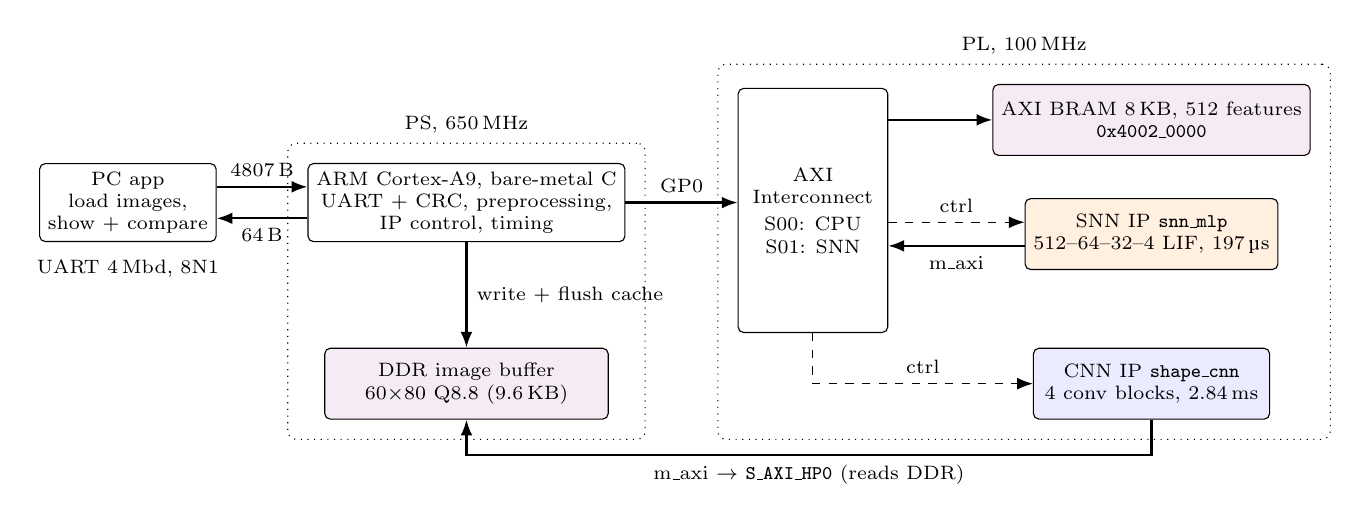
\begin{tikzpicture}[font=\scriptsize,
  blk/.style={draw, rounded corners=2pt, align=center, minimum height=9mm, inner sep=3pt, fill=white},
  arr/.style={-{Latex[length=2mm]}, thick},
  ctl/.style={-{Latex[length=2mm]}, dashed},
  reg/.style={draw, dotted, rounded corners=3pt, inner sep=2.5mm}]
\node[blk, minimum width=20mm] (pc) at (0,0.4) {PC app\\load images,\\show + compare};
\node[blk, minimum width=36mm] (cpu) at (4.3,0.4) {ARM Cortex-A9, bare-metal C\\UART + CRC, preprocessing,\\IP control, timing};
\node[blk, minimum width=36mm, fill=violet!8] (ddr) at (4.3,-1.9) {DDR image buffer\\$60{\times}80$ Q8.8 (9.6\,KB)};
\node[blk, minimum width=19mm, minimum height=31mm] (ic) at (8.7,0.3) {AXI\\Interconnect\\[2pt]S00: CPU\\S01: SNN};
\node[blk, minimum width=30mm, fill=violet!8] (bram) at (13.0,1.45) {AXI BRAM 8\,KB, 512 features\\\texttt{0x4002\_0000}};
\node[blk, minimum width=30mm, fill=orange!12] (snn) at (13.0,0.0) {SNN IP \texttt{snn\_mlp}\\512--64--32--4 LIF, 197\,\textmu s};
\node[blk, minimum width=30mm, fill=blue!8] (cnn) at (13.0,-1.9) {CNN IP \texttt{shape\_cnn}\\4 conv blocks, 2.84\,ms};
\draw[arr] ([yshift=2mm]pc.east) -- node[above]{4807\,B} ([yshift=2mm]cpu.west);
\draw[arr] ([yshift=-2mm]cpu.west) -- node[below]{64\,B} ([yshift=-2mm]pc.east);
\node[below=1mm of pc] {UART 4\,Mbd, 8N1};
\draw[arr] (cpu) -- node[right]{write + flush cache} (ddr);
\draw[arr] (cpu) -- node[above]{GP0} (cpu.east -| ic.west);
\draw[arr] (ic.east |- bram) -- (bram.west);
\draw[ctl] ([yshift=1.5mm]ic.east |- snn.west) -- node[above]{ctrl} ([yshift=1.5mm]snn.west);
\draw[arr] ([yshift=-1.5mm]snn.west) -- node[below]{m\_axi} ([yshift=-1.5mm]ic.east |- snn.west);
\draw[ctl] (ic.south) |- node[pos=0.75, above]{ctrl} (cnn.west);
\draw[arr] (cnn.south) -- ++(0,-0.45) -| node[pos=0.25, below]{m\_axi $\to$ \texttt{S\_AXI\_HP0} (reads DDR)} (ddr.south);
\begin{scope}[on background layer]
\node[reg, fit=(cpu)(ddr), label={[font=\scriptsize]above:PS, 650\,MHz}] {};
\node[reg, fit=(ic)(bram)(snn)(cnn), label={[font=\scriptsize]above:PL, 100\,MHz}] {};
\end{scope}
\end{tikzpicture}
\caption{System overview: both accelerators in one bitstream, selected per request by the CPU.
CNN reads its input from DDR via \texttt{HP0}; SNN reads its features from an AXI BRAM through the
CPU's interconnect (dashed: AXI-Lite control).}
\end{figure}

\textbf{Division of work.} Apart from sending raw 8-bit images and showing and evaluating
the answers, the PC does nothing. All the rest runs on the board: the CPU receives and checks
each frame, converts the pixels to Q8.8 for the CNN or computes the 512 spike features for the
SNN, and starts the IP over AXI-Lite. After polling \texttt{ap\_done} it reads the prediction
and the scores and sends them back, together with timings from the global timer (325\,MHz).

\textbf{Memory arrangement.} Each IP gets its input in a different way. For the CNN, the
CPU writes the Q8.8 image (9.6\,KB) to a DDR buffer, flushes the data cache and passes the
address, and the IP fetches the image as an AXI master through \texttt{S\_AXI\_HP0} into its
own BRAM. SNN features instead go through \texttt{M\_AXI\_GP0} into an 8\,KB AXI BRAM at
\texttt{0x4002\_0000}. Because the BRAM controller has only one slave port, the SNN's
\texttt{m\_axi} port is connected to a second input (\texttt{S01}) of the same interconnect,
so CPU and SNN see the BRAM at the same address. Getting there took a while: Vivado's
connection automation had put the SNN's master port on an interconnect that led nowhere, and
the SNN hung until we wired it by hand. Results come back in AXI-Lite registers.

\textbf{UART protocol.} PS UART0 runs over USB at 4\,000\,000\,Bd, 8N1, without flow
control. Requests have the form \texttt{AA 55 | cmd | len(u16) | payload | CRC-16}, responses
\texttt{55 AA | cmd | status | len | payload | CRC-16} (CRC-16/CCITT, init \texttt{0xFFFF},
little endian). Besides CNN, SNN and BOTH (each carrying the 4800-byte image) there are ECHO and
INFO. An inference reply holds the board's receive time and, per network, the class,
preprocessing time, IP time and 4 scores (26\,B). ECHO was useful early on, to test the image
transfer before any IP was integrated.

% ==================================================================
\section{Results}
\begin{table}[h]
\centering\small
\begin{tabular}{lcc}
\toprule
 & CNN & SNN \\
\midrule
Test accuracy: software (float) & \cnnKerasAcc\,\% & \snnFloatAcc\,\% \\
Test accuracy: integer / fixed-point reference & -- & \snnIntAcc\,\% \\
Test accuracy: on board & \cnnBoardAcc\,\% & \snnBoardAcc\,\% \\
\quad per class (circle / square / triangle / fig-8) & 100 / 100 / 100 / 100 & 98.0 / 97.7 / 97.7 / 98.3 \\
HLS latency @100\,MHz & \cnnLatCyc\ cyc (\cnnLatUs\,\textmu s) & \snnLatCyc\ cyc (\snnLatUs\,\textmu s) \\
Measured IP time (start$\to$done) & \cnnIpUs\,\textmu s & \snnIpUs\,\textmu s \\
CPU preprocessing & \cnnPreUs\,\textmu s & \snnPreUs\,\textmu s \\
Throughput, IP only & 352 img/s & 5\,076 img/s \\
Throughput, IP + preprocessing & 320 img/s & 494 img/s \\
LUT / FF & 9\,843 / 8\,503 & 3\,638 / 3\,348 \\
BRAM36 eq.\ / DSP & 68 / 53 & 11 / 8 \\
Power (Vivado, post-route, IP) & 0.266\,W & 0.056\,W \\
Energy per inference (IP) & 755\,\textmu J & 11\,\textmu J \\
\bottomrule
\end{tabular}
\caption{CNN vs.\ SNN on the same 1200 test images (300 per class), one bitstream, 100\,MHz,
timing met (WNS +0.257\,ns). Whole design: 15\,584 LUT (29\,\%), 81 BRAM tiles (58\,\%),
61 DSP (28\,\%), 1.76\,W on chip (1.26\,W of it the ARM processing system).}
\label{tab:res}
\end{table}

\textbf{Communication overhead.} A request is 4807 bytes and a BOTH reply 64 bytes, or
\SI{12.2}{ms} on the wire at 4\,Mbd. Just receiving an image takes the board \uartMs\,ms. On
the PC, a full BOTH round trip measures \rttMs\,ms (31 images/s), of which only 5.2\,ms is
preprocessing and inference. That makes the UART $4\times$ slower than the CNN and $60\times$
slower than the SNN, with the remaining 13.5\,ms going to USB latency and the Python code on
the PC. ECHO on its own (50 images, 0 errors) gave a 42.8\,ms round trip.

\textbf{Discussion and future work.} In accuracy the CNN wins (100\,\% against 97.9\,\%,
with the SNN's 25 errors spread over all classes). Everywhere else it loses: $2.7\times$ the
LUTs, $6.6\times$ the DSPs, $70\times$ the energy per image, and $14\times$ slower. Most of the
SNN's speed comes from its binary spikes. Since each spike is just a 0 or a 1, the hidden layers
only add weights instead of multiplying. We also skip zero inputs in the first layer, and with
$T=1$ the network runs just once. Its weak point is the hand-made encoder. Computing the spike
features takes 1.8\,ms on the CPU, which is $9\times$ the time of the SNN itself. So end to end,
the SNN is only $1.5\times$ faster than the CNN. Moving the encoder into the FPGA would close that
gap. Since
the UART is the real bottleneck, the biggest gains lie in the link: Ethernet or the USB-OTG
port, compressed images, or sending only the 512 features (1\,KB instead of 4.8\,KB). DMA with
double buffering could also receive the next image while the current one is processed.
We could also try $T>1$ with rate or temporal coding, which might trade some SNN speed for accuracy.

% ==================================================================
\section{Bonus: swapping the networks with DFX}
We only ever need one network at a time, so for the bonus we put both of them in the same
area of the FPGA and swap between them while the board is running (Dynamic Function eXchange).
For this to work, both networks have to fit the same slot. We gave each IP a small wrapper so
they have exactly the same registers and the same memory port, which means the SNN now reads
its features from DDR like the CNN instead of from the BRAM. Each network also writes an id
number, so the firmware can tell which one is loaded. The shared area covers the lower two
thirds of the chip and is sized for the CNN, since it is the bigger one.

A swap loads a 4.2\,MB partial bitstream over JTAG and takes about 2.5\,s, while the CPU
keeps running. The first time we tried it, the board froze right after the swap. While the
area is being rewritten its outputs change randomly, and that locked up the AXI bus. Resetting
the FPGA logic after every swap fixed it (a DFX decoupler would be the proper fix). Both
versions meet timing at 100\,MHz. After each swap the networks give the same accuracy and IP
time as in the normal design (Table~\ref{tab:dfx}).

\begin{table}[h]
\centering\small
\begin{tabular}{lcc}
\toprule
 & CNN loaded & SNN loaded \\
\midrule
Test accuracy on board & 100\,\% (100 images) & 97.92\,\% (1200 images) \\
Measured IP time & 2\,840\,\textmu s & 197\,\textmu s \\
LUT / BRAM36 eq.\ / DSP in the shared area & 10\,221 / 68 / 53 & 3\,948 / 14.5 / 8 \\
Power on chip (whole design) & 1.72\,W & 1.49\,W \\
Time to swap (JTAG) & \multicolumn{2}{c}{about 2.5\,s} \\
\bottomrule
\end{tabular}
\caption{DFX results on the PYNQ-Z2. The shared area has room for 36\,400 LUT, 100 BRAM tiles
and 160 DSP; the fixed part around it uses only about 865 LUT. The CNN uses a few more LUTs than in Table~\ref{tab:res} because of its wrapper.}
\label{tab:dfx}
\end{table}

\end{document}
